\documentclass{article}

\usepackage{parskip}
\usepackage{graphicx}
\usepackage[margin=0.5in]{geometry}

\title{Visualisation}
\author{xfdg93}

\begin{document}
\maketitle

\section*{Problem 1}
\begin{figure}
	\centering
	\includegraphics[width=10cm]{gen.png}
	\caption{Image generated by Problem 1}
	\label{fig:gen}
\end{figure}
\begin{figure}
	\centering
	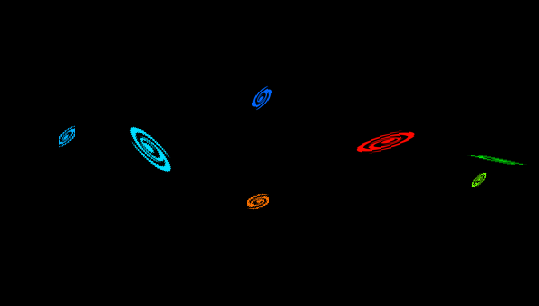
\includegraphics[width=10cm]{croppedgen.png}
	\caption{Close up of image generated by Problem 1}
	\label{fig:closefig}
\end{figure}

vis.py generates a number (set to 100) of galaxies with random $x$, $y$ and $z$ coordinates in the space $0<x,y,z<1$.
It also generates a random rotation and size.
It uses the Z coordinate to generate a colour, by using the Z coordinate as a ratio between 240 and 1, e.g $H = 240(1-z)$.
This value of $H$ is then used as a hue, and the saturation and intensity are set to 1.
This colour in the HSI colour space is converted to a colour in the RGB colour space.
It then uses the Pillow python library to render the given image to a PNG file (Figure \ref{fig:gen}, \ref{fig:closefig}), with the generated location, size, rotation and colour.

The HSI colour space is ideal for the rainbow colour scale as red corresponds to 0, green to 120, and blue to 240, so a smooth scale from 240 to 0 passes through the rainbow colour scale from blue to red.

\section*{Problem 2}

vis.py uses cv2's Simple Blob Detector to detect the location of the galaxies on the image.
First it uses the Simple Blob Detector to get a list of the locations of images.
It then collects the area around the detected blob. The size of the area collected depends on the size of the blob reported by cv2.
It then takes a weighted average of the hue of each pixel in the area, weighting pixels closest to the center of the blob higher.
It then uses this hue to extract the $z$ coordinate, using the inverse of the transformation made when generating the image, e.g. $z = 1-(\frac{H}{240})$

It then stores in an array, for each galaxy, the three coordinates, as well as an image of the collected area around the galaxy, except with all pixels sufficiently far away from the hue of the galaxy set to black. This means that galaxies extremely close together would not show up on each others images.

\section*{Problem 3}

Figure \ref{fig:v1:front} shows my visualisation from the front, figure \ref{fig:v1:side} shows it from the side, and figure \ref{fig:v1:scale} shows it with some scaling factor applied.

\begin{figure}
	\centering
	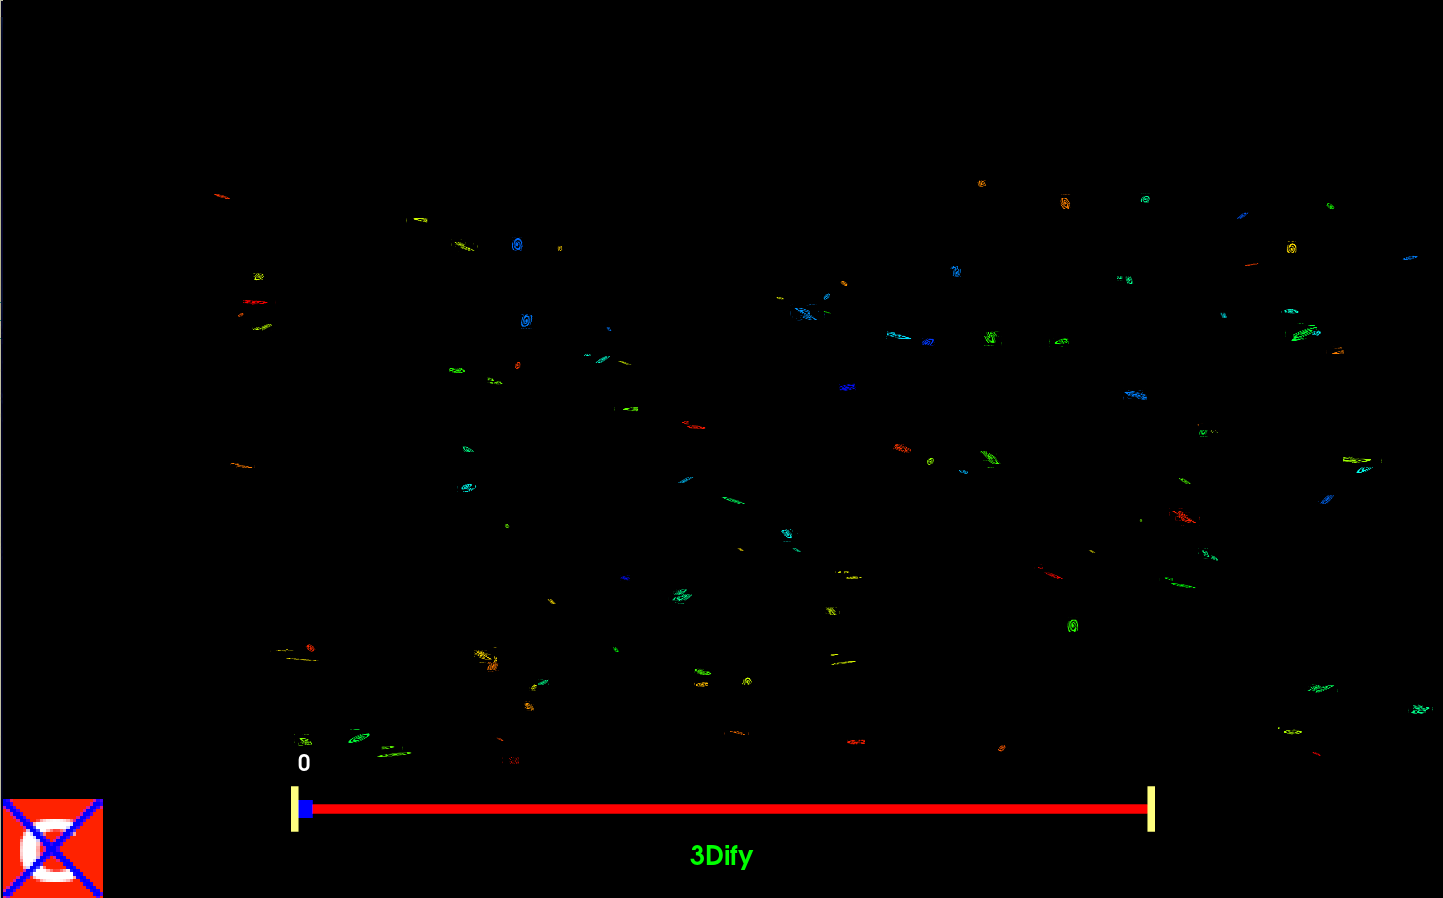
\includegraphics[width=10cm]{2022-04-16-212252_1443x898_scrot.png}
	\caption{Visualisation 1 from the front}
	\label{fig:v1:front}
\end{figure}
\begin{figure}
	\centering
	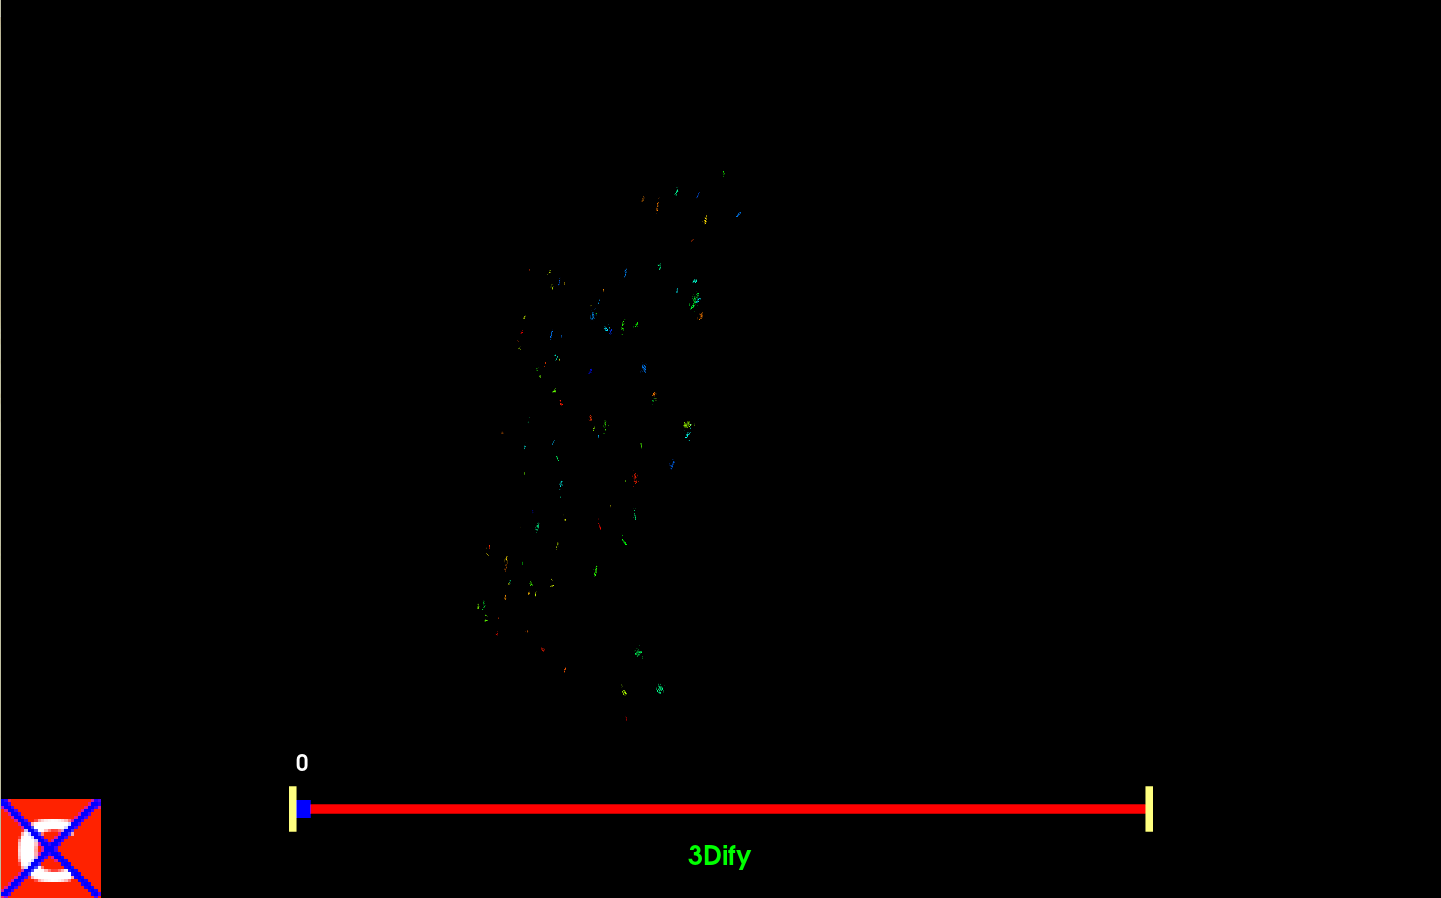
\includegraphics[width=10cm]{2022-04-16-212305_1441x898_scrot.png}
	\caption{Visualisation 1 from the side}
	\label{fig:v1:side}
\end{figure}
\begin{figure}
	\centering
	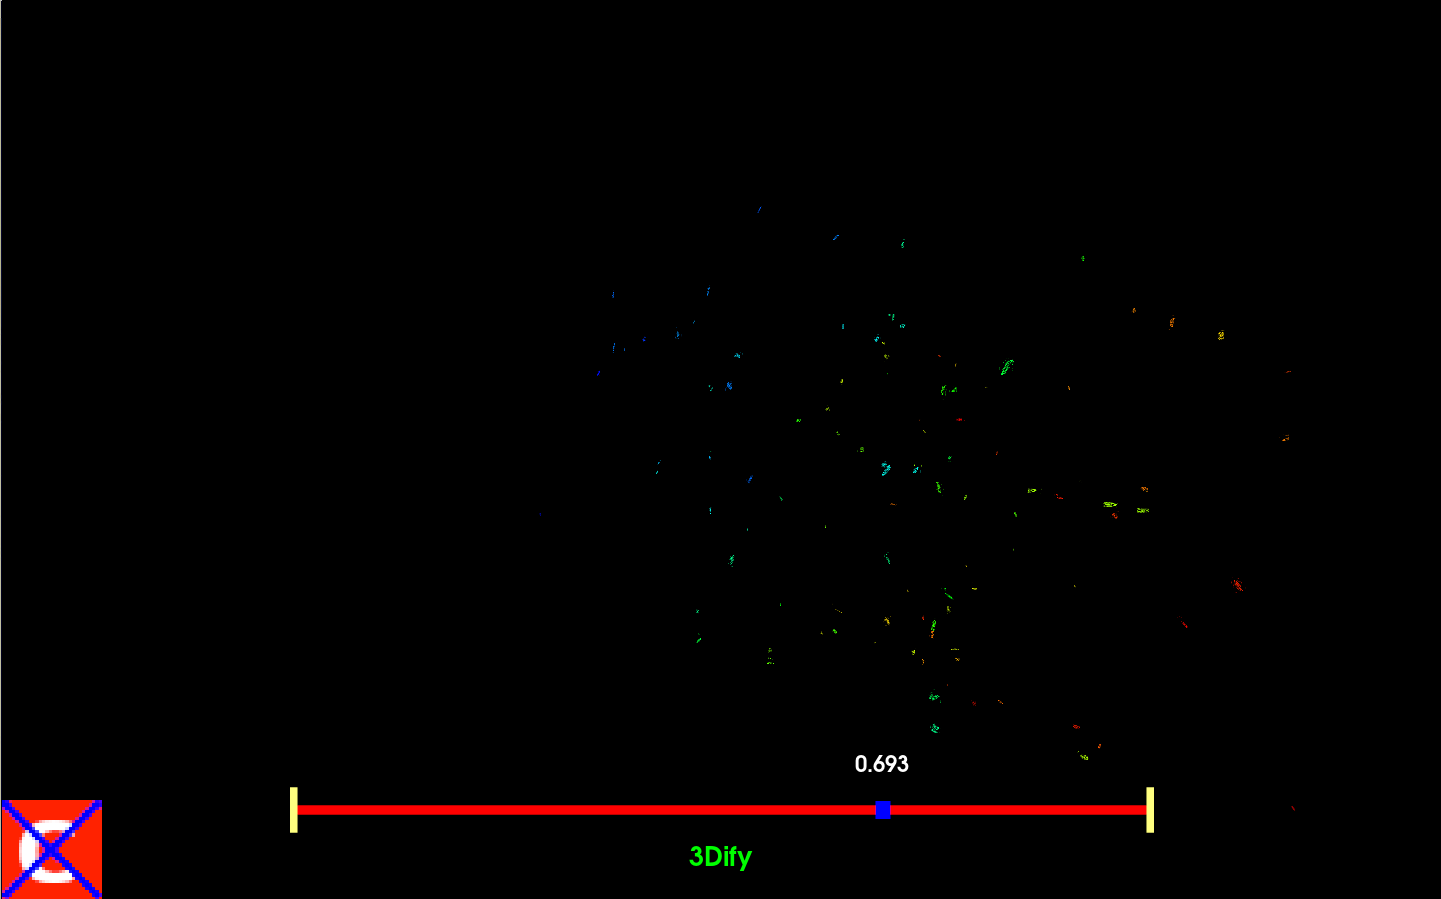
\includegraphics[width=10cm]{2022-04-16-212318_1441x899_scrot.png}
	\caption{Visualisation 1 from the side with scale factor applied}
	\label{fig:v1:scale}
\end{figure}
\begin{figure}
	\centering
	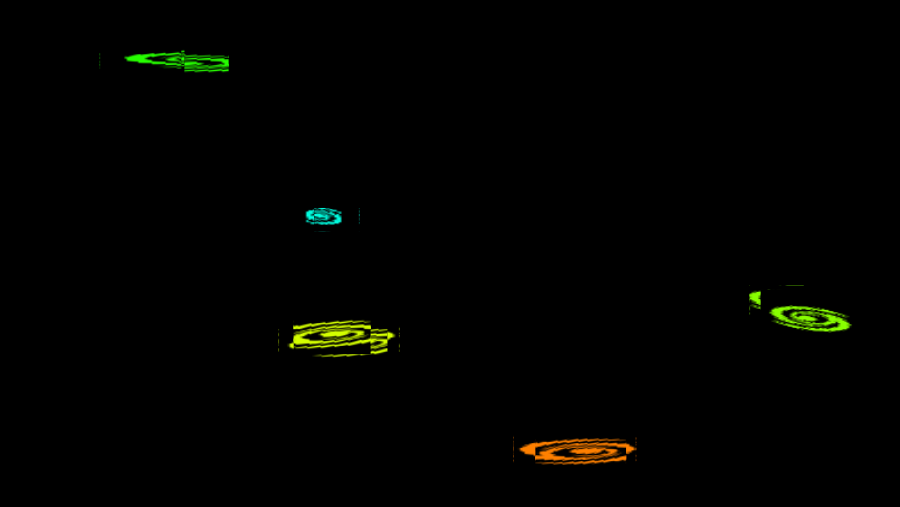
\includegraphics[width=10cm]{2022-04-16-212857_900x507_scrot.png}
	\caption{Visualisation 1 closeup}
	\label{fig:v1:close}
\end{figure}


\section*{Problem 4}

For problem 4, vis.py demonstrates that, despite the stars and galaxies in star constellations looking close by from one angle, they are actually many times that distance apart when viewed from the side.
I decided to use white for the lines in the constellations,  as it is often used in maps of the constellations, and therefore is already assosiated with constellations for the viewer.
Many of the more recognisable constelations are a tree structure, and all are connected graphs, and so in order to simulate this, vis.py generates tree structured contellations.


\begin{figure}
	\centering
	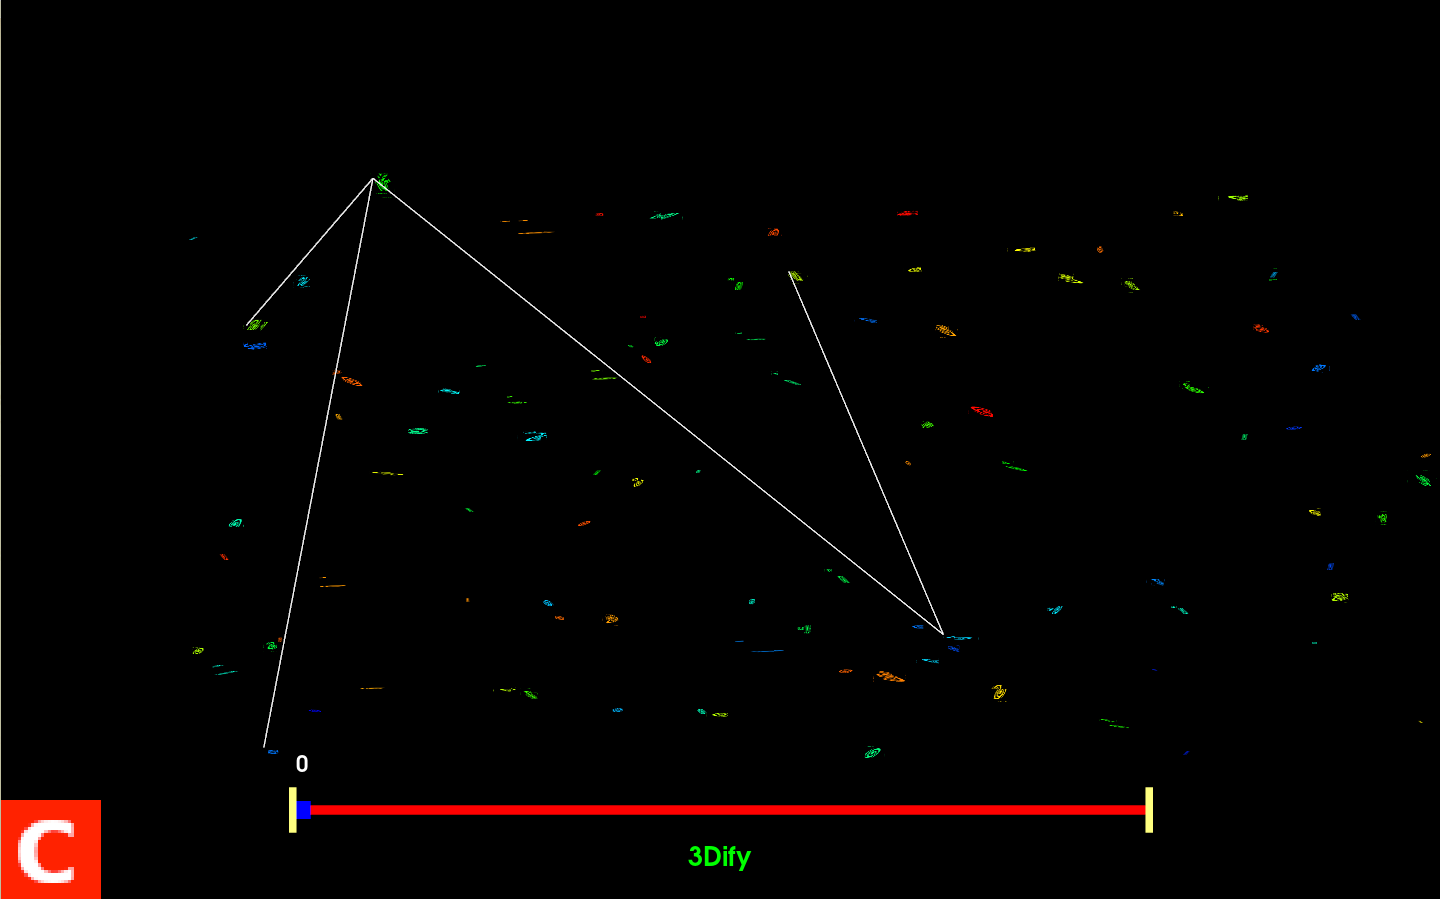
\includegraphics[width=10cm]{2022-04-16-212350_1440x899_scrot.png}
	\caption{Visualisation 2 from the front}
	\label{fig:v2:front}
\end{figure}
\begin{figure}
	\centering
	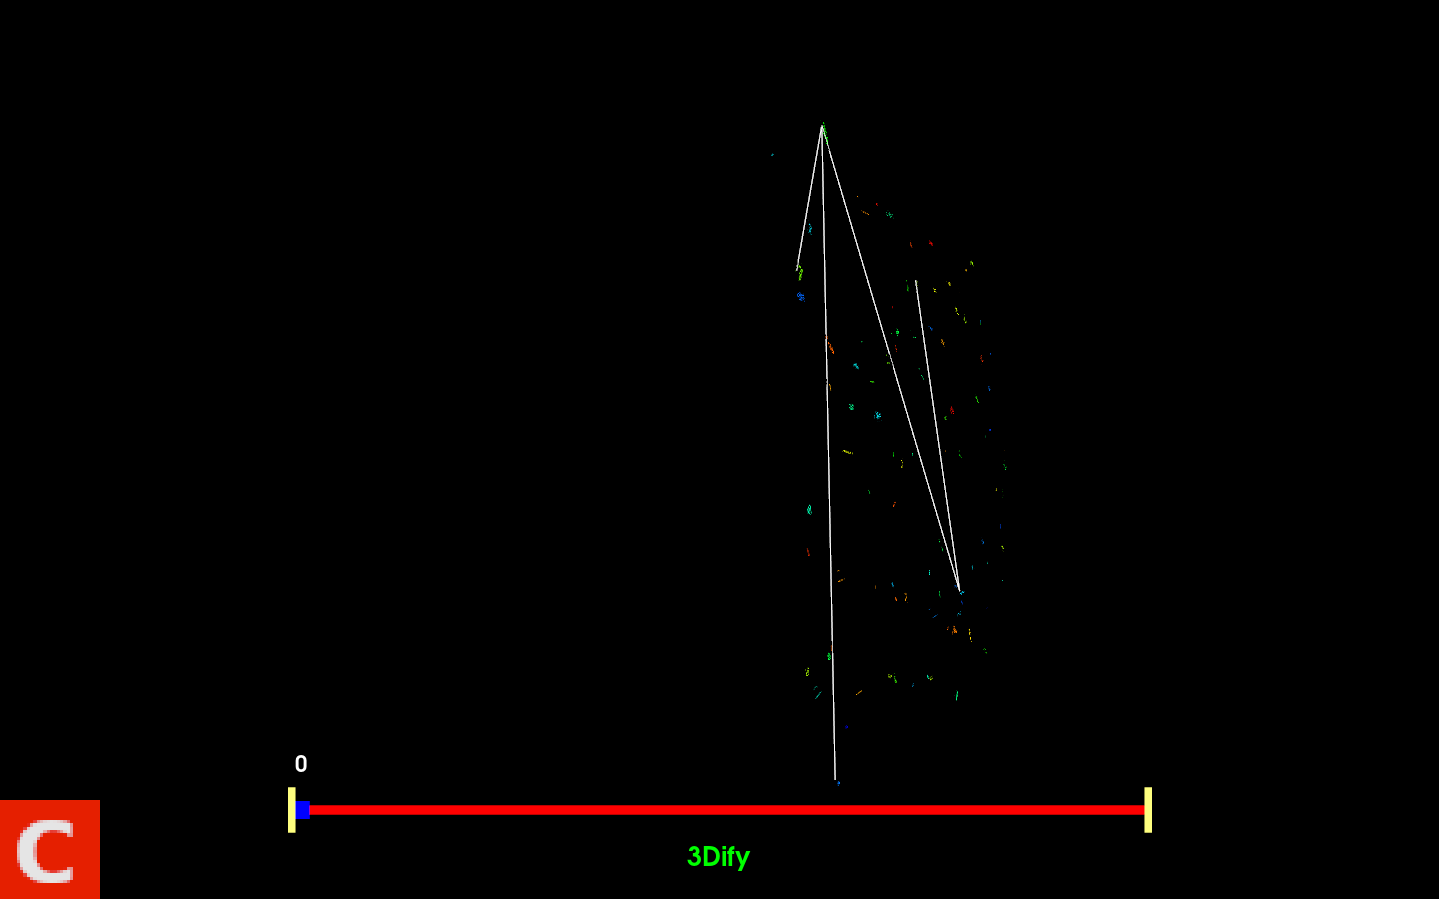
\includegraphics[width=10cm]{2022-04-16-212359_1439x899_scrot.png}
	\caption{Visualisation 2 from the side}
	\label{fig:v2:side}
\end{figure}
\begin{figure}
	\centering
	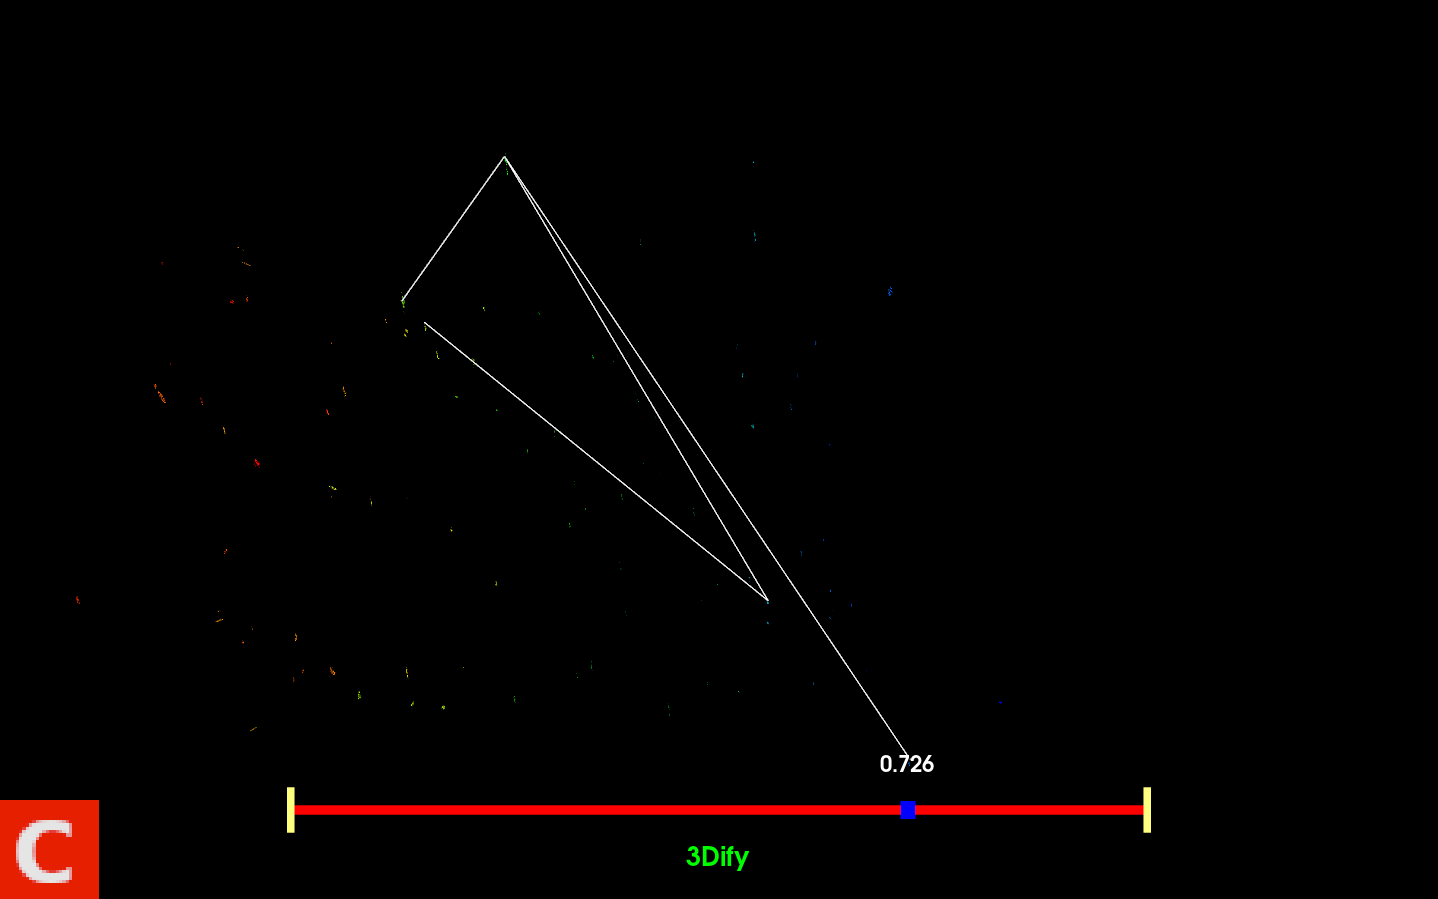
\includegraphics[width=10cm]{2022-04-16-212411_1438x899_scrot.png}
	\caption{Visualisation 2 from the side with scale factor applied}
	\label{fig:v2:scale}
\end{figure}




\end{document}
